\section{Nozzle mechanics, hardware, and kinematics}
\label{sec:hardware}
\subsection{Two materially different ways to deliver hot glass}
Reservoir extrusion and laser-heated filament deposition solve different hardware problems. In the former, a crucible provides an inventory of conditioned melt and a nozzle meters a continuous cord. In the latter, a solid feedstock carries material to a small hot zone; deposition occurs after local softening or melting. Separating these architectures prevents an inappropriate comparison between a furnace setpoint and a laser's nominal power. Both are direct hot-glass routes, but their thermal inventory, material residence time, attainable feature size, and interruption behavior differ.

The historical MIT G3DP apparatus demonstrated transparent reservoir-fed material extrusion with a heated receiving chamber. Its institutional project description specifies an upper kiln cartridge and a lower annealing chamber. The later G3DP2 paper describes three-zone thermal control and four-axis motion, alongside a demonstration of assembled architectural columns. These publications establish feasibility and increasingly integrated process control; they do not establish that every printed component is suitable for structural service without qualification.\cite{acad_klein2015,acad_mitproject,acad_inamura2018}

\subsection{Flow resistance and nozzle selection}
As a deliberately simplified design model, steady Newtonian flow through an isothermal cylindrical bore gives
\begin{equation}
 Q=\frac{\pi r^4}{8\eta L}\Delta p,\qquad
 \Delta p\simeq \rho g H+\Delta p_{\mathrm{act}},
 \label{eq:nozzleflow}
\end{equation}
where $r$ is bore radius, $L$ is bore length, $H$ is melt head, and $\Delta p_{\mathrm{act}}$ is any imposed pressure. The expression excludes entrance losses, capillary pressure, temperature gradients, slip, and a partially obstructed outlet. It should be treated as a scaling law for engineering estimates, not as a calibrated G3DP flow model. Its useful implications are immediate: doubling radius increases predicted flow sixteenfold; doubling viscosity halves predicted flow; and emptying a gravity-fed reservoir changes output even when the heater setpoint stays fixed.

For a slowly varying nozzle profile the corresponding approximation is
\begin{equation}
 \Delta p_{\mathrm{visc}}=\frac{8Q}{\pi}
 \int_0^L\frac{\eta[T(z)]}{r(z)^4}\,\mathrm{d}z.
\end{equation}
The coldest narrow section can therefore dominate pressure loss. A heater mounted above the tip cannot by itself prove that the issuing glass has the intended viscosity. A practical experimental calibration would weigh deposited glass against time while recording head height, nozzle temperatures, dwell time, and glass batch. A flow map should include warm-up and restart transients rather than only the best steady segment. This calibration protocol is a proposal of this review.

Refractory ceramic and precious-metal wet-contact parts require different qualification. MIT's historical project page uses the wording alumina--zircon--silica for its nozzle; that description should not be generalized to all apparatus versions. Heraeus documents platinum and platinum-alloy glass-manufacturing components and emphasizes that alloy choice depends on the glass and required purity. In particular, its optical-glass guidance favors rhodium-free platinum materials where coloration matters, while Pt--Rh alloys appear in other demanding glass-processing applications. Thus ``platinum--rhodium is always best'' is not a supportable design rule. Supplier information is evidence of materials availability and engineering considerations, not independent proof of a particular printer's nozzle life.\cite{acad_mitproject,acad_heraeus}

\subsection{Motion control is also material control}
Ignoring shrinkage and evaporation, conservation of mass relates deposited area $A_b$ to travel speed $U$ through $A_b\simeq Q/U$. A corner slowdown therefore increases local cross-section unless flow changes at the same time. Conversely, acceleration can thin a bead and reduce contact with the previous layer. Discontinuous paths add a second problem: molten glass stored downstream of a metering mechanism can continue moving after its command stops. Designing a path as a continuous loop reduces repeated starts, although it restricts accessible topology.

These observations motivate a proposed controller with separate estimation of thermal state, material delivery, and position. A geometric planner should specify the desired cross-section and contact location; a deposition controller should translate these into speed and flow commands with actuator delays. The controller should monitor actual bead shape rather than interpreting successful motor motion as successful deposition. Height feedback is particularly valuable because small layer errors accumulate and change the physical gap between nozzle or hot zone and the growing part.

Laser filament systems remove the need for a large nozzle filled with molten silica. Von Witzendorff and colleagues demonstrated quartz-fiber deposition using a CO$_2$ laser and translating substrate. Liu and colleagues subsequently examined symmetric laser heating and bonding of approximately $196\,\mu$m fused-silica filament; their multilayer experiment used $200\,\mu$m nominal layers. These are research operating conditions, not a universal printer resolution.\cite{acad_witzendorff2018,acad_liu2022} Their significance is that energy delivery, filament feed, and substrate motion jointly determine fusion. Nominal laser power alone cannot specify the delivered energy density without optical coupling, beam geometry, feedstock diameter, and speed.

\subsection{Proposed hardware qualification sequence}
\begin{figure}[htbp]
\centering
\begin{subfigure}[c]{.40\linewidth}\centering
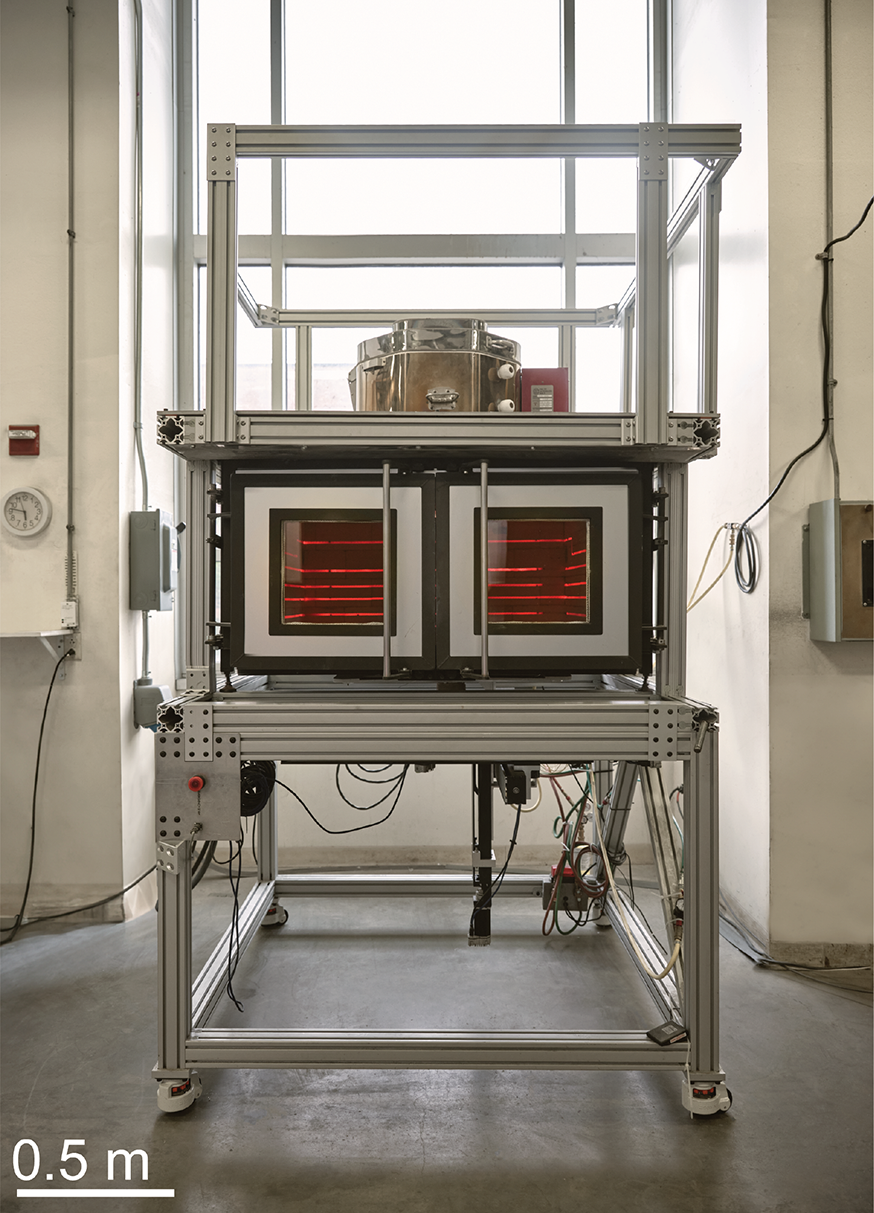
\includegraphics[height=62mm]{figures/Massimino2024_Figure1.png}
\caption{G3DP3 reservoir-fed apparatus.}
\end{subfigure}\hfill
\begin{subfigure}[c]{.55\linewidth}\centering
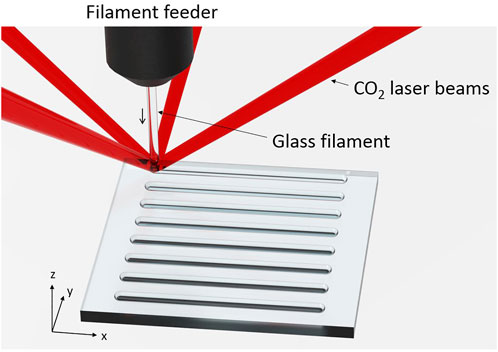
\includegraphics[width=\linewidth]{figures/Liu2022_Figure1.jpg}
\caption{Four-beam laser filament heating.}
\end{subfigure}
\caption{Contrasting thermal architectures. Left: Massimino et al. (2024), Figure 1, showing the G3DP3 build chamber below the furnace/crucible, \href{https://doi.org/10.1007/s40940-024-00279-8}{original article}. Right: Liu, Oriekhov and Fokine (2022), Figure 1, \href{https://doi.org/10.3389/fmats.2022.978861}{original article}. Both images reproduced unmodified under \href{https://creativecommons.org/licenses/by/4.0/}{CC BY 4.0}. The drawing and photograph are not to a common scale.}
\end{figure}
A useful acceptance sequence begins with stationary thermal characterization, proceeds to single tracks and starts/stops, then to turns, stacked walls, and representative enclosed geometries. At each stage, assess both geometric error and material integrity. For nozzles, inspect bore growth, adhering deposits, inclusions in the glass, and leakage at joints. For filament systems, inspect diameter variation, feed damage, and direction-dependent heating. These tests are recommended engineering controls rather than published capability claims. They make a machine specification reproducible: a build envelope without its hot-zone clearances, thermal stability, and supported path geometry is an incomplete description of usable manufacturing capacity.
